\documentclass[11pt, a4paper, twoside, openright]{book} %draft

\usepackage{graphicx,color}
\usepackage{amssymb, amsmath, array}
\usepackage{cite}
\usepackage[T1]{fontenc}

\usepackage{listings}
\usepackage{color}
\usepackage{dirtytalk}

\graphicspath{{illustrations/}}

\begin{document}

% Example of title page for the projects carried out within DEDIS
% Copied from lasec

% Simply include it in your mastex tex file:
%        % Example of title page for the projects carried out within DEDIS
% Copied from lasec

% Simply include it in your mastex tex file:
%        % Example of title page for the projects carried out within DEDIS
% Copied from lasec

% Simply include it in your mastex tex file:
%        \input{cover}


% Updated October 2016


\newcommand{\logoepfl}[0]{
  \begin{center}
    
\includegraphics[width=4cm]{logo_epfl_coul.eps}
  \end{center}
  \vspace{0.3cm}
  \hrule
}
\newcommand{\project}[1]{
  \begin{center}
    \large{#1}
  \end{center}
  \vspace{1cm}
}
\newcommand{\department}[1]{
  \begin{center}
    \large{#1}
  \end{center}
}
\newcommand{\lab}[1]{
  \begin{center}
    \large{#1}
  \end{center}
}
\newcommand{\supervisor}[3]{
  \begin{center}
    \begin{normalsize}{
        \bf #1}\\#2\\#3
    \end{normalsize}
  \end{center}
}
\renewcommand{\author}[1]{
  \begin{center}
    \Large{#1}
  \end{center}
  \vspace{0.5cm}
}
\renewcommand{\title}[1]{
  \vspace{3cm}
  \begin{center}
    \huge{#1}
  \end{center}
  \vspace{1.7cm}
}
\renewcommand{\date}[2]{
  \begin{center}
    \normalsize{#1 #2}
  \end{center}
  \vspace{0.5cm}
}


\thispagestyle{empty}


% begin title page
  \logoepfl
  
  \title{Web-Frontend for Cothority}

  \author{Bastian Nanchen}
  \department{School of Computer and Communication Sciences}
  \lab{Decentralized and Distributed Systems lab}
  \project{Semester Project}

  \date{December}{2016}

  \begin{center}
    \begin{tabular}{cc}
      \begin{tabular}{p{4.0cm}}
        \supervisor{Responsible}{Prof.Bryan Ford}{EPFL / DEDIS}
      \end{tabular}&
      \begin{tabular}{p{4.0cm}}
        \supervisor{Supervisor}{Linus Gasser}{EPFL / DEDIS}
      \end{tabular}
    \end{tabular}
  \end{center}

% end title page



% Updated October 2016


\newcommand{\logoepfl}[0]{
  \begin{center}
    
\includegraphics[width=4cm]{logo_epfl_coul.eps}
  \end{center}
  \vspace{0.3cm}
  \hrule
}
\newcommand{\project}[1]{
  \begin{center}
    \large{#1}
  \end{center}
  \vspace{1cm}
}
\newcommand{\department}[1]{
  \begin{center}
    \large{#1}
  \end{center}
}
\newcommand{\lab}[1]{
  \begin{center}
    \large{#1}
  \end{center}
}
\newcommand{\supervisor}[3]{
  \begin{center}
    \begin{normalsize}{
        \bf #1}\\#2\\#3
    \end{normalsize}
  \end{center}
}
\renewcommand{\author}[1]{
  \begin{center}
    \Large{#1}
  \end{center}
  \vspace{0.5cm}
}
\renewcommand{\title}[1]{
  \vspace{3cm}
  \begin{center}
    \huge{#1}
  \end{center}
  \vspace{1.7cm}
}
\renewcommand{\date}[2]{
  \begin{center}
    \normalsize{#1 #2}
  \end{center}
  \vspace{0.5cm}
}


\thispagestyle{empty}


% begin title page
  \logoepfl
  
  \title{Web-Frontend for Cothority}

  \author{Bastian Nanchen}
  \department{School of Computer and Communication Sciences}
  \lab{Decentralized and Distributed Systems lab}
  \project{Semester Project}

  \date{December}{2016}

  \begin{center}
    \begin{tabular}{cc}
      \begin{tabular}{p{4.0cm}}
        \supervisor{Responsible}{Prof.Bryan Ford}{EPFL / DEDIS}
      \end{tabular}&
      \begin{tabular}{p{4.0cm}}
        \supervisor{Supervisor}{Linus Gasser}{EPFL / DEDIS}
      \end{tabular}
    \end{tabular}
  \end{center}

% end title page



% Updated October 2016


\newcommand{\logoepfl}[0]{
  \begin{center}
    
\includegraphics[width=4cm]{logo_epfl_coul.eps}
  \end{center}
  \vspace{0.3cm}
  \hrule
}
\newcommand{\project}[1]{
  \begin{center}
    \large{#1}
  \end{center}
  \vspace{1cm}
}
\newcommand{\department}[1]{
  \begin{center}
    \large{#1}
  \end{center}
}
\newcommand{\lab}[1]{
  \begin{center}
    \large{#1}
  \end{center}
}
\newcommand{\supervisor}[3]{
  \begin{center}
    \begin{normalsize}{
        \bf #1}\\#2\\#3
    \end{normalsize}
  \end{center}
}
\renewcommand{\author}[1]{
  \begin{center}
    \Large{#1}
  \end{center}
  \vspace{0.5cm}
}
\renewcommand{\title}[1]{
  \vspace{3cm}
  \begin{center}
    \huge{#1}
  \end{center}
  \vspace{1.7cm}
}
\renewcommand{\date}[2]{
  \begin{center}
    \normalsize{#1 #2}
  \end{center}
  \vspace{0.5cm}
}


\thispagestyle{empty}


% begin title page
  \logoepfl
  
  \title{Web-Frontend for Cothority}

  \author{Bastian Nanchen}
  \department{School of Computer and Communication Sciences}
  \lab{Decentralized and Distributed Systems lab}
  \project{Semester Project}

  \date{December}{2016}

  \begin{center}
    \begin{tabular}{cc}
      \begin{tabular}{p{4.0cm}}
        \supervisor{Responsible}{Prof.Bryan Ford}{EPFL / DEDIS}
      \end{tabular}&
      \begin{tabular}{p{4.0cm}}
        \supervisor{Supervisor}{Linus Gasser}{EPFL / DEDIS}
      \end{tabular}
    \end{tabular}
  \end{center}

% end title page


\begingroup
\let\cleardoublepage\clearpage
\tableofcontents
\endgroup

\chapter{Introduction}
\section{History}
%First present the work at Dedis Cothority and Cosi
Distributed cryptography spreads the operation of a cryptosystem among a group
of servers in a fault-tolerant way~\cite{definition}.\\
The DEDIS lab at EPFL created the Cothority project, which implements decentralized
and distributed cryptographic protocols.\\

TODO:presentation of the report!!!!!!!!!!!!!!!!!!!!!!!!!!!!!!!!!

%Myself
\section{Aims and Goals}
The goal of this semester project is to furnish a web-interface to the Cothority
project.\\
The aims stated at a summer meeting with Mr.Linus Gasser are to create an
interface with status' conodes, be able to send a file for a collective signature
and to verify a signature.\\


\chapter{Analysis}
The first part of the semester project was to acquire knowledge in JavaScript and
HTML and become familiar with the JQuery library. For delivering a skeleton of
the website before the beginning of the semester.\\
Next thing to settle was the communication between the website and a conode.
The JavaScript Web APIs contain all the necessary to handle this problem.
The object Websocket~\cite{websocketPage} offers all the tools to create a
communication between a browser and a server.\\

TODO:presentation of the .proto files!!!!!!!!!!!!!!!!!!!!!!!!!!!!!!!!!


The Cothority's approach for serializing structured data is a Google's Protobuf-like.
As said on the website of Google's Protobuf:\say{Protocol buffers are a flexible,
efficient, automated mechanism for serializing structured data - think XML, but
smaller, faster, and simpler.}~\cite{protobufDefi}.\\
Taking this into account and knowing that Google's Protobuf doesn't support generated
code in JavaScript, the choice was made on the library protobuf.js~\cite{protobufjs}.
It is a pure JavaScript implementation of Google's Protobuf. It uses the same format
of .proto file.

\begin{lstlisting}[caption={example of .proto file}, captionpos=b]
 message Foo{
            required bytes a = 1;
            required bytes b = 2;
        }
\end{lstlisting}

%talk about the implementation of the Status Part
\section{Status part}
The JavaScript Web APIs contain all the necessary to handle the communication
part. The object Websocket~\cite{websocketPage} offers all the tools to create a
communication between a browser and a server and send/receive data. All the elements send to conodes are .proto files.\\
First it is necessary to establish the connection. A connection is established
with each conode.\\
An empty .proto file is send in a Blob object containing the .proto file in bytes.\\

\begin{lstlisting}[caption={empty .proto file}, captionpos=b]
  message Request {
  }
\end{lstlisting}

The request being sent the webpage waits for a response. The response will be the
status of the concerning conode. It is received as a .proto file.

\begin{lstlisting}[caption={response .proto file}, captionpos=b]
  message ServerIdentity{
    				required bytes public = 1;
    				required bytes id = 2;
    				required string address = 3;
    				required string description = 4;
				}

  message Response {
    				map<string, Status> system = 1;
    				optional ServerIdentity server = 2;

				    message Status {
        				map<string, string> field = 1;
    				}
				}
\end{lstlisting}

The response is is a map with field corresponding to another message format, which
is a map of a string with a string. Each key corresponding to an element of the conode's
status (port number, hostname, number of bytes received and sent,\ldots) and each field
to its value.\\
%Mettre une subsection?????????????
\subsection{Promise API}
That being said, the response message is triggered by our opening socket message. Therefore the
response message will be asynchronous.\\
To tackle the asynchronous problem, the introduction of the Promise object in JavaScript must be
made. First it is important to know that JavaScript is single threaded. It means
that if a code snippet is waiting on data, the thread can't be waiting on it and doesn't execute
the remaining part of the code. In that case JavaScript program would be very slow.
So through the history of JavaScript many tools were created to handle asynchronous programs.
Like callback functions that was widely used, but widely disliked too. It even has a nickname:\say{Callback Hell}.\\

\begin{lstlisting}[caption={Example of Callback Hell with its typical pyramid shape}, captionpos=b]
  fs.readdir(source, function (err, files) {
  if (err) {
    console.log('Error finding files: ' + err)
  } else {
    files.forEach(function (filename, fileIndex) {
      console.log(filename)
      gm(source + filename).size(function (err, values) {
        if (err) {
          console.log('Error identifying file size: ' + err)
        } else {
          console.log(filename + ' : ' + values)
          aspect = (values.width / values.height)
          widths.forEach(function (width, widthIndex) {
            height = Math.round(width / aspect)
            console.log('resizing ' + filename + 'to ' + height + 'x' + height)
            this.resize(width, height).write(dest + 'w' + width + '_' + filename, function(err) {
              if (err) console.log('Error writing file: ' + err)
            })
          }.bind(this))
        }
      })
    })
  }
})
\end{lstlisting}
\leavevmode \\
Other libraries (jQuery) begun implementing promises to help developers overcome the \say{Callback Hell}.
This eventually leads ECMAScript 6 to adopt The Promise API~\cite{promise} natively in JavaScript~\cite{ecmaPromise}.
The object Promise allows to retrieve a value in the \say{future}.
\\
\begin{lstlisting}[caption={Structure of a Promise}, captionpos=b]
  var promise = new Promise(function(resolve, reject) {
    // asynchronous snippet code
    if (/*everything goes well*/) {
      resolve(/*result of async element*/);
    } else {
      reject(/*result of async part*/);
    }
  });
\end{lstlisting}
\leavevmode \\
A callback function needs to be passed at the Promise's constructor. This function
will have two parameters. The resolve function will be called if everything worked in
the asynchronous part, otherwise the reject function will be called.\\
In the case of this semester project, the resolve function will return the response
.proto file containing all the status data from the conode.\\

\leavevmode \\

\subsection{Generator}
To handle the Promise returned the project will use another feature of ECMAScript 6 called a Generator.
It's a new kind of function. It can be paused in the middle and resumed later. Of course,
other parts of the code are running during the pause.\\

\begin{lstlisting}[caption={Structure of a generator function}, captionpos=b]
  function* foo() {
    var x = yield 1;
  }
  \end{lstlisting}
\leavevmode \\
The \say{*} marks the function as a generator one. The other different element of
the code snippet is the keyword:\say{yield}. \say{yield \underline{\hspace{1cm}} is called a \say{yield expression} (and not a statement) because when we restart the generator, we will send a value back in, and whatever we send in will be the computed result of that yield \underline{\hspace{3cm}} expression.}
~\cite{yieldExpression}. The function will stop when it encounters the \say{yield} keyword.
Whenever (if ever) the generator is restarted, the \say{yield 1} expression will send \say{1} back.
The part following the \say{yield} keyword is the expression that will be returned.\\

 \begin{lstlisting}[caption={Restart of a generator function}, captionpos=b]
   var a = foo();
   a.next();
 \end{lstlisting}
 \leavevmode \\
The call to the \say{next()} method will execute the generator (from the last \say{yield}) to the next encounter of a \say{keyword} (if there is any).\\
Returning to the project's code, a generator function is used with the function returning a Promise object.\\

\begin{lstlisting}[caption={Extract from the project's code}, captionpos=b]
  function* generator() {
        // some code
        var message = yield websocket_status(7003);
        listNodes.push(nodeCreation(message));
        // some code
    });
}
\end{lstlisting}
\leavevmode \\
The function \say{websocket\_status()} returns a Promise object. The generator function
stops when reaching \say{websocket\_status()}. \say{The main strength of generators is that they provide a single-threaded, synchronous-looking code style, while allowing you to hide the asynchronicity away as an implementation detail.}~\cite{runGenerator}.
The idea is to \say{yield} out promises and let them restart the generator function when
they are fulfilled. To do so we need to create a new function that will control the generator function's iterator.\\
\begin{lstlisting}[caption={Extract from the project's code~\cite{runGenerator}}, captionpos=b]
  function runGenerator(g) {
    let iterator = g();
    (function iterate(message) {
        let ret = iterator.next(message);

        if (!ret.done) {
            ret.value.then(iterate);
        }
    })();
  }
\end{lstlisting}
\leavevmode \\
This function takes a generator function as parameter. The \say{iterator} function
is the generator function. The inner-function \say{iterate()} will look if a promise
returns the value \say{message} from \say{iterator.next(message)}. If not (\say{ret.done} == false), the function
will iterate again.\\

\subsection{Implementation}
Now all the elements needed are presented, it only remains to do it for each node.\\

\begin{lstlisting}[caption={Extract from the project's code reaching conodes at port 7003, 7005 and 7007}, captionpos=b]
  runGenerator(function* generator() {
        listNodes = [];
        let message = yield websocket_status(7003);
        listNodes.push(nodeCreation(message));
        message = yield websocket_status(7005);
        listNodes.push(nodeCreation(message));
        message = yield  websocket_status(7007);
        listNodes.push(nodeCreation(message));
        // some code
    });
\end{lstlisting}
\leavevmode \\
As said above the \say{websocket\_status()} function returns a Promise object. Thus
the generator function \say{generator()} will \say{yield} before each \say{websocket\_status()} call.
The generator function is given in parameter to the \say{runGenerator()} function.\\
The Promise API, the generator function and the util function \say{runGenerator()} allow to hide
the asynchronous part of the code. It is more readable and more modular.\\

% Google Chrome with async

% Not final part if recursive method done [BEGIN]
Then it only remains to do it for each node.
% Not final part if recursive method done [END]

\section{Signature part}
The semester project must implement the possibility to send a file for a collective signature
and to verify a signature.


In the Cothority project the signature is a Schnorr signature, which is a zero-knowledge proof presented
by Mr.Schnorr in 1989. It is \say{based on the intractability of certain discrete logarithm problems}~\cite{wikiSchnorr}.\\
In the part where the user can send a file and sign it by the conodes,
the website needs to calculate the aggregate key using the public keys of the conodes.
More details will be presented in the Implementation subsection.\\
The private and the public key used in the Cothority project require the usage of
the Edwards-curve Digital Signature Algorithm (edDSA).
\say{edDSA is a variant of Schnorr's signature system with Twisted Edwards curves.}~\cite{edDSA}.
The Cothority project uses Ed25519, which is an instantiation of EdDSA, for the
public key signature. Ed25519 has some interesting aspect as a fast key generation,
small keys and an high security level~\cite{ed25519}.\\
% TODO deplace the above paragraph?!?!?!

\subsection{Send a file for a collective signature}
\subsubsection{Analysis}

\subsubsection{Implementation}
The implementation of the HTML part is straightforward. It needs an input tag to
submit a file and all the collapse-thing is managed by the Bootstrap framework~\cite{bootstrap}.\\

\begin{figure}[ht!]
\centering
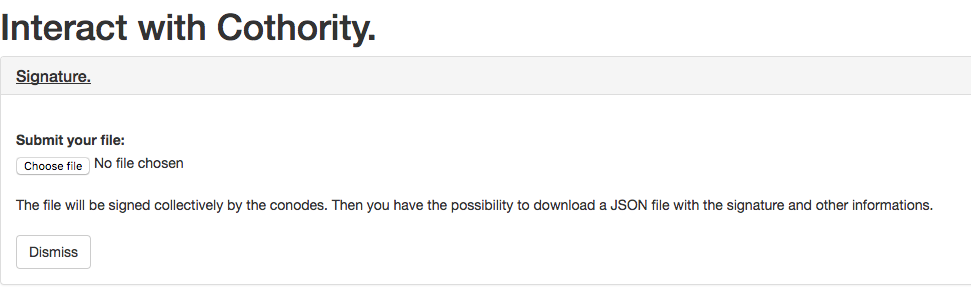
\includegraphics[width=125mm]{verification_signature.jpg}
\caption{Interface}
\end{figure}
\leavevmode \\

The file submitted is read as an ArrayBuffer~\cite{ArrayBuffer}. The Promise APIs,
a generator function and the \say{runGenerator()} function are used to deal with
the asynchronous part of submitting a file. The reading of the file is returned
inner a Promise object in a generator function that is given in paramter to the
\say{runGenerator()} util function (go to subsection n°2.1 for more details on
the manner to tackle the asynchronous part).\\ % TODO come back for the number of the subsection

Afterward the file needs to be signed. To do so the program uses two libraries
protobuf.js~\cite{protobufjs} that was introduced before and js-nacl~\cite{jsnacl}.
As said on the library's GitHub page: \say{A high-level Javascript API wrapping an Emscripten-compiled libsodium, a cryptographic library based on NaCl. Includes both in-browser and node.js support.}.
NaCl (Networking and Cryptography library) is a software library written in C for
network communication, encryption, decryption, signatures,\ldots~\cite{nacl}. Its
goal is to \say{provide all of the core operations needed to build higher-level cryptographic tools}~\cite{nacl}.
Little disclaimer NaCl is pronounced "salt".
In this semester project the js-nacl library is employed % TODO rester ici!!!!!!

The user has the possibility to submit a file and download a JSON file containing
the signature's file, the filename, the date, the aggregate key and the hash of the file.\\
When the file has been uploaded to the website, it remains to contact a conode to sign it.\\
\begin{lstlisting}[caption={.proto file}, captionpos=b]
  message ServerIdentity{
            required bytes public = 1;
            required bytes id = 2;
            required string address = 3;
            required string description = 4;
        }

        message Roster {
            optional bytes id = 1;
            repeated ServerIdentity list = 2;
            optional bytes aggregate = 3;
        }

        message SignatureRequest {
            required bytes message = 1;
            required Roster roster = 2;
        }

        message SignatureResponse {
            required bytes hash = 1;
            required bytes signature = 2;
            required bytes aggregate = 3;
        }
\end{lstlisting}
\leavevmode \\


%talk about the problem encountered with Linus


% talk about the graphic part at the end
% each 3 seconds

\begingroup
\let\cleardoublepage\clearpage
\bibliography{report}{}
\bibliographystyle{ieeetr}
\endgroup

\end{document}
